\documentclass{article} % For LaTeX2e
\usepackage[legalpaper, margin=0.16in]{geometry}
\usepackage{amsmath}
\usepackage{amsfonts,dsfont}
\usepackage{amssymb}
\usepackage[ruled,vlined]{algorithm2e}

\usepackage{graphicx}
\usepackage{caption}
\usepackage{subcaption}
\usepackage{xcolor}
\usepackage{siunitx}

\begin{document}

\begin{figure}
	\centering
	\captionsetup{labelformat=empty}
	\begin{subfigure}[b]{0.3\textwidth}
		%% trim=left bottom right top
		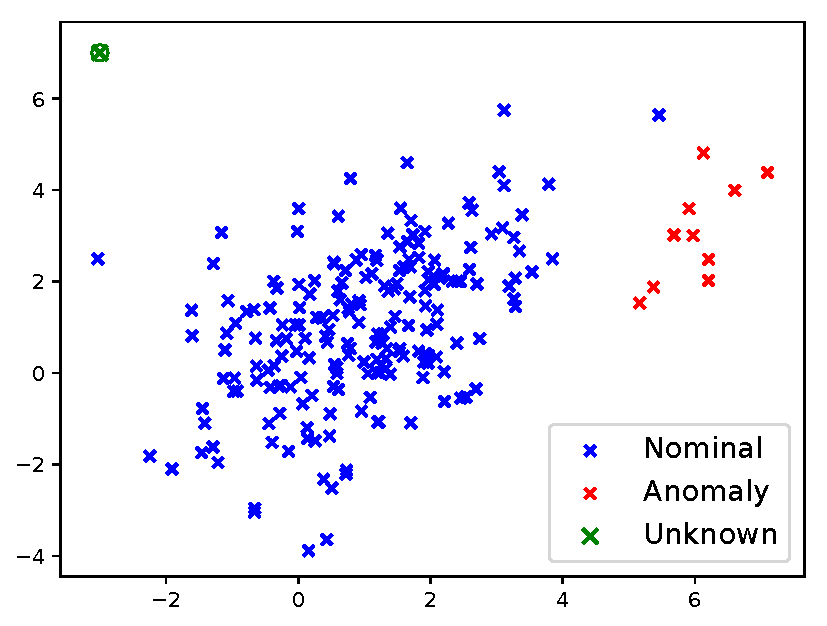
\includegraphics[width=\textwidth, clip=true, trim=0mm 0mm 0mm 0mm]{avc_dataset_5}
		\caption{Dataset with labeled examples}
		\label{fig:dataset}
	\end{subfigure}
	\begin{subfigure}[b]{0.3\textwidth}
		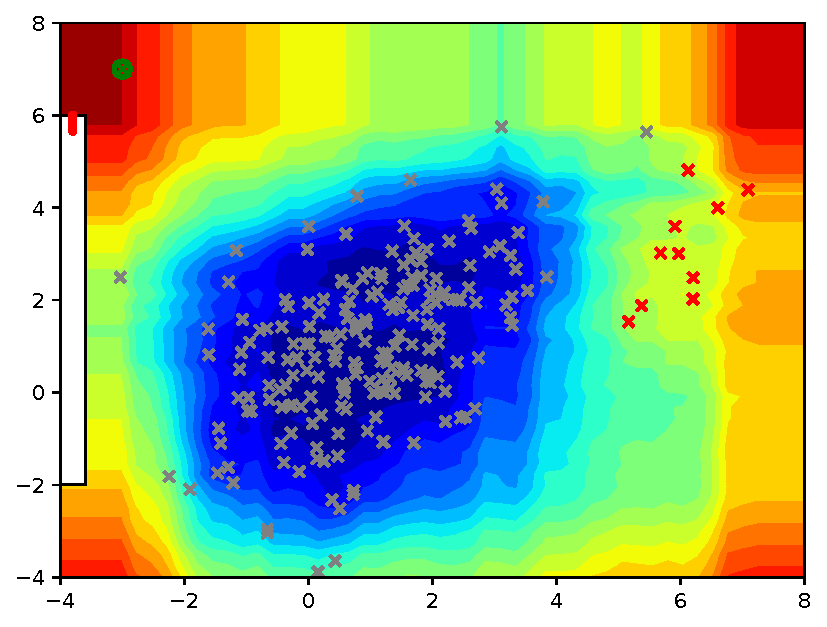
\includegraphics[width=\textwidth, clip=true, trim=0mm 0mm 0mm 0mm]{avc_dataset_5_anomaly}
		\caption{Score contours for anomaly detector}
		\label{fig:aad}
	\end{subfigure}
    \begin{subfigure}[b]{0.3\textwidth}
    	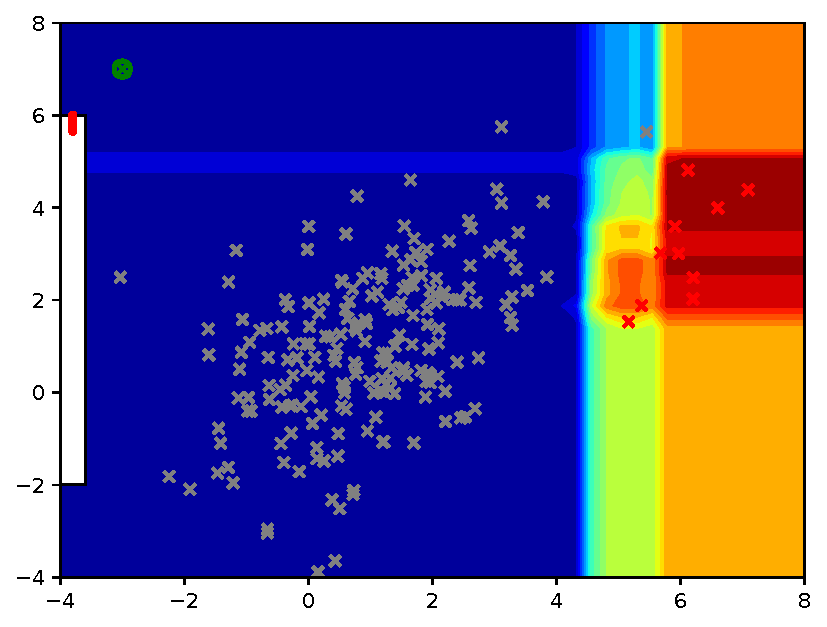
\includegraphics[width=\textwidth, clip=true, trim=0mm 0mm 0mm 0mm]{avc_dataset_5_classifier}
    	\caption{Score contours for classifier}
    	\label{fig:rf}
    \end{subfigure}\\
    \begin{subfigure}[b]{0.3\textwidth}
    	%% trim=left bottom right top
    	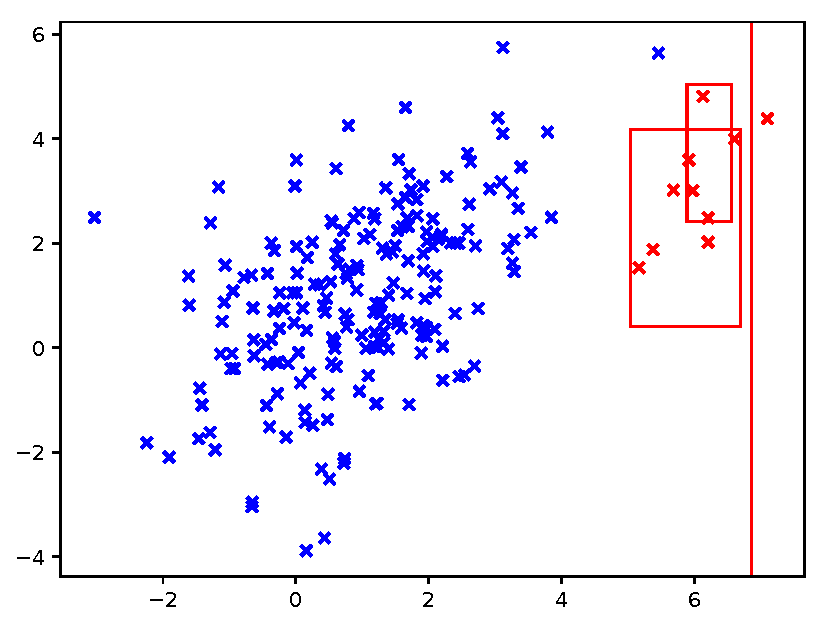
\includegraphics[width=\textwidth, clip=true, trim=0mm 0mm 0mm 0mm]{avc_dataset_5_anomaly_descriptions}
    	\caption{Descriptions (AAD)}
    	\label{fig:dataset}
    \end{subfigure}
    \begin{subfigure}[b]{0.3\textwidth}
    	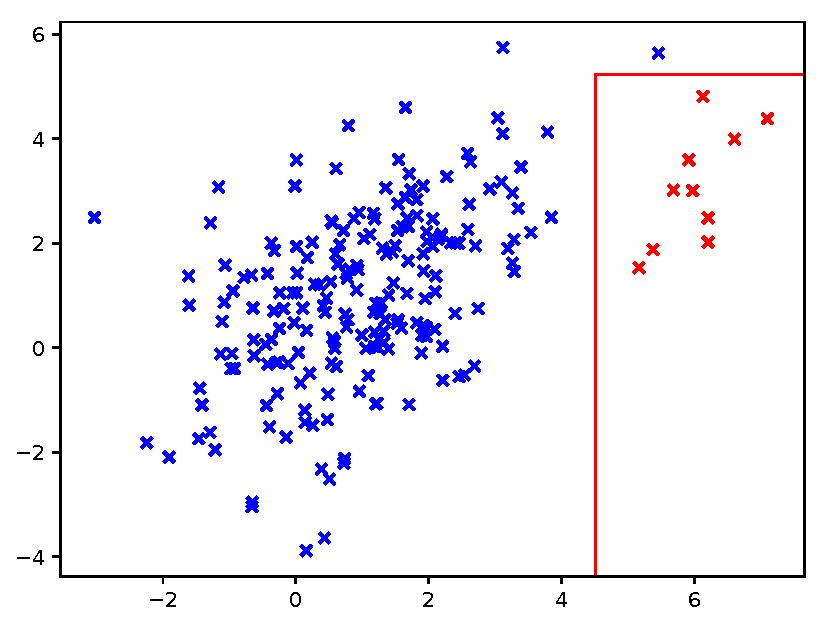
\includegraphics[width=\textwidth, clip=true, trim=0mm 0mm 0mm 0mm]{avc_dataset_5_decision_tree_descriptions}
    	\caption{Descriptions (Decision Tree Classifier)}
    	\label{fig:aad}
    \end{subfigure}
    \begin{subfigure}[b]{0.3\textwidth}
    	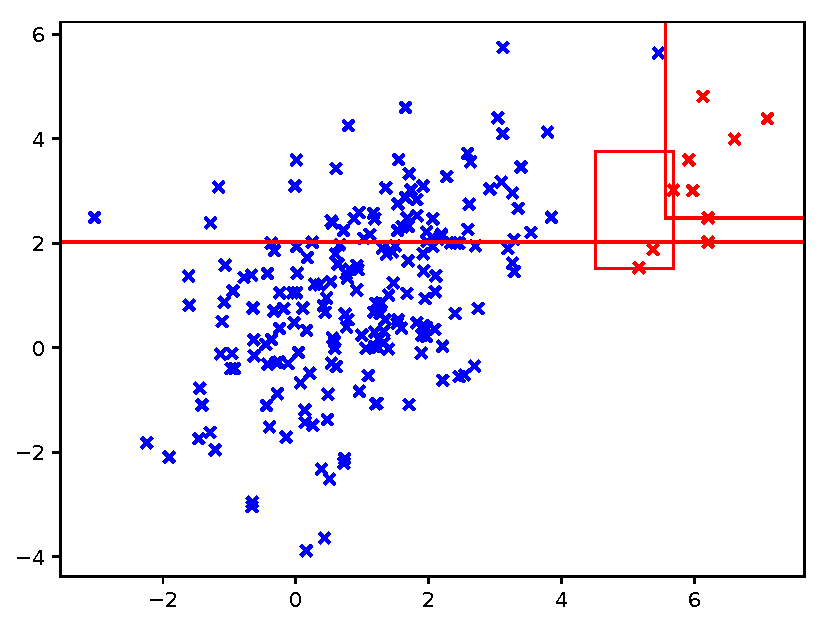
\includegraphics[width=\textwidth, clip=true, trim=0mm 0mm 0mm 0mm]{avc_dataset_5_random_forest_descriptions}
    	\caption{Descriptions (Random Forest Classifier)}
    	\label{fig:rf}
    \end{subfigure}
	\caption{Anomaly detector (AAD) vs. Classifier (Random Forest) when labeled data is available. {\bf (a)} Shows the labeled dataset. Only the point marked in green at the top left is unlabeled. {\bf (b)} Shows the anomaly score contours when the anomaly detector (AAD) was trained with the labeled instances (i.e., \textbf{ensemble weights were tuned to take the labels into account}). {\bf (c)} Shows the probability contours for the anomaly class when a classifier was employed. In both (b) and (c), \textcolor{red}{\textbf{red}} corresponds to \textit{more anomalous}, and \textcolor{blue}{\textbf{blue}} corresponds to \textit{more nominal}. Although we employed a \textit{Random Forest} (RF) classifier, it learned an almost linear classifier. All points to the left of $x=4.5$ (approx.) will be classified as \textbf{nominal} by the classifier, including the unlabeled point marked in \textcolor{green}{\textbf{green}}. In contrast, the \textcolor{green}{\textbf{green}} point will be classified as \textbf{anomaly} by the anomaly detector. Since the classifier learns a \textit{decision boundary} between the two classes, it only checks which side of the boundary the instance is on before classifying it. On the other hand, most i.i.d point-based anomaly detectors (like in this example) are sensitive to the \textit{data density}; instances which are in sparse regions are more likely be flagged as anomalies by default. \textbf{Whether to choose an anomaly detector or a classifier is application dependent and there are likely use cases for both types of behaviors.} The bottom row illustrates the anomaly descriptions generated by {\bf(d)}~AAD; {\bf(e)}~Decision~Tree~(DT); and {\bf(f)}~RF. Since both DT and RF are tree-based, we employed the same strategy as the one for generating compact descriptions with AAD. For DT, which comprises of only a single tree which partitions the entire data exclusively, this naturally corresponds to simple rule-extraction. Since the anomalies are well-separated and fully labeled, DT works well. In case of AAD and RF, there are many overlapping subspaces and the description algorithm tries to minimize the total volume which covers all labeled anomalies. Therefore, the selected subspaces are smaller. In all cases, the subspaces could probably be pruned further based on the location of the anomalies, for example, in {\bf (e)}, the lower limit could be moved to $y=1.0$ (approx.) instead of $y=-\infty$. The descriptions might help in a more systematic analysis. For example, (d) shows that the anomalies are contained in three subspaces with $1$, $7$, and $3$ instances; we could perhaps distribute the analysis effort between $2$ or $3$ analysts, or analyze the $7$ instances which belong to the same subspace on priority.}
	\label{fig:regression}
\end{figure}

\end{document}
